\begin{center}
	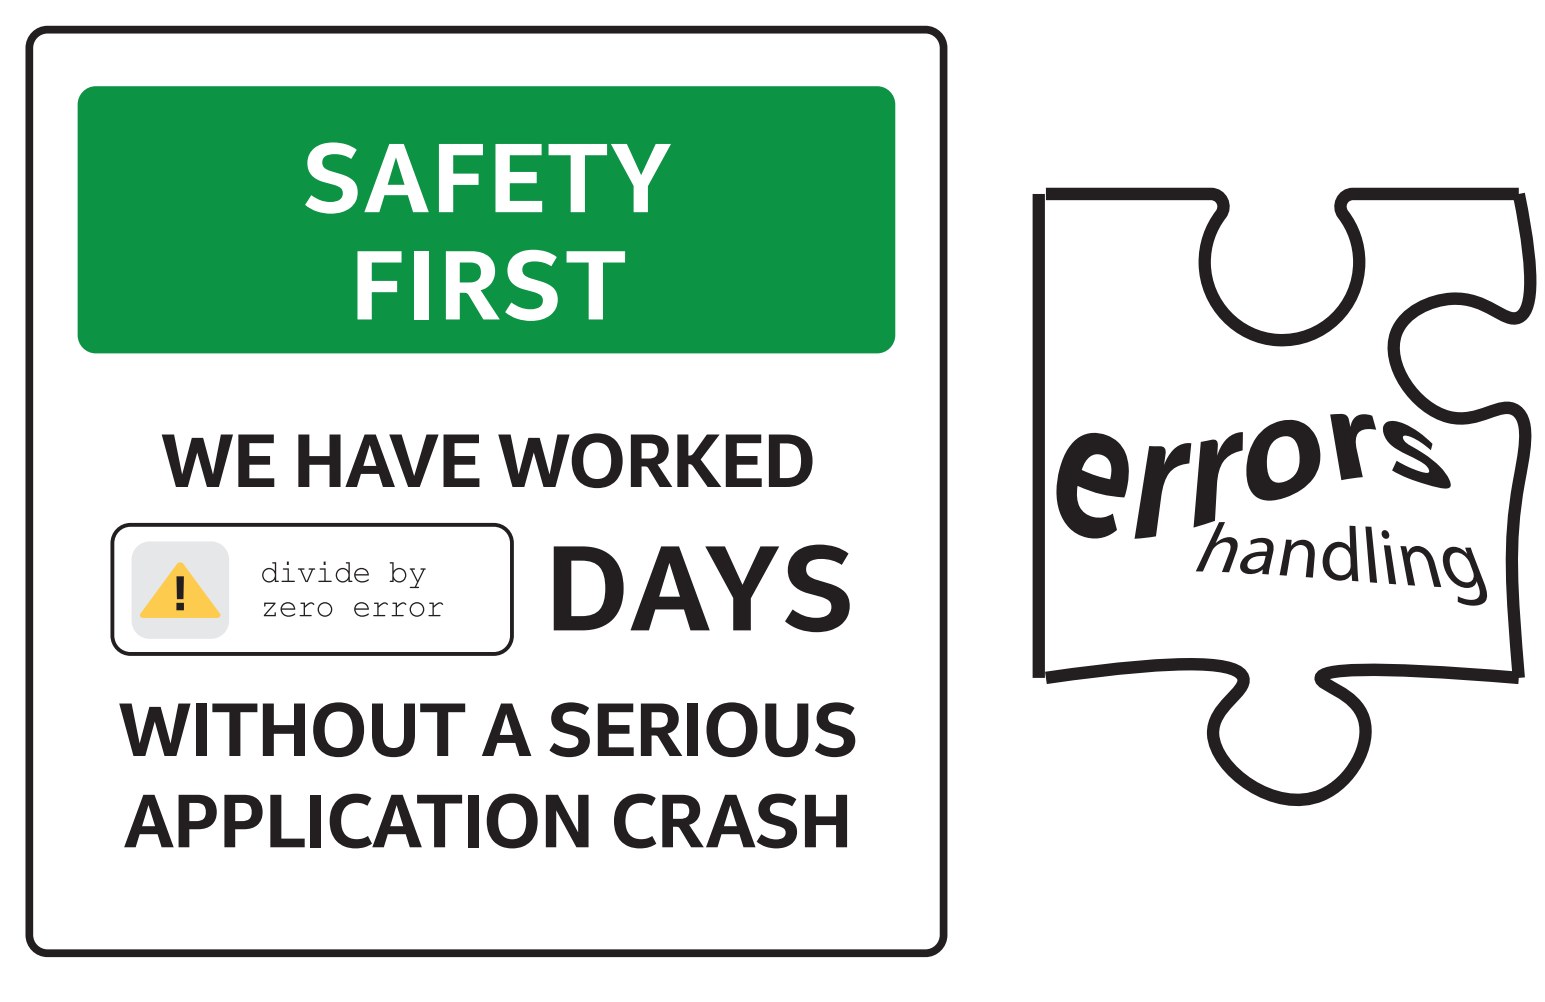
\includegraphics[width=0.5\textwidth]{content/chapter-5/images/1}
\end{center}

阿加莎·克里斯蒂(Agatha Christie)在1969年写道:“如果尝试与计算机所能做到的事情相比,人为错误根本算不了什么。”错误处理机制可以捕获其他可能犯的错误,可以使用错误处理来处理可能由于某些原因发生的情况。\par

开发应用期间,检测和处理错误很有帮助(在项目中的其他开发者也会犯错误),更重要的是,其在稳定和安全的程序和库中扮演着关键角色。本章将一起来了解SYCL中可用的错误处理机制,以便能够了解我们有哪些选择,以及如何构建应用程序。\par

本章概述了SYCL中的同步和异步错误,描述了不处理错误时,应用程序的行为,并深入研究了SYCL处理异步错误的机制。\par